\subsection{Intergratie testen}
Alle belangrijke interacties tussen de componenten zijn getest door middel van intergratie testen.
Deze testen zijn ook gemaakt in xUnit een van de geimplementeerde testen is te zien in figuur \ref{fig:IntergrationTest}.
In het voorbeeld is te zien dat er gebruik wordt gemaakt van het mocken van de repository.
Mocken is het gebruiken van een \qw{nep} implementatie van de gebruikte interface. 
hierdoor kan je aangeven wat je specifiek van een methode terug verwacht.
Omdat dat er gebruik gemaakt wordt van het repository pattern is het makkelijk om de database te mocken.
Verder is er een overzicht te zien van alle testen in figuur \ref{fig:OverviewUnitTests}.


\whitespace[2]
\begin{graphic}
	\captionsetup{type=figure}
	\caption{Geimplementeerde intergratie test}
	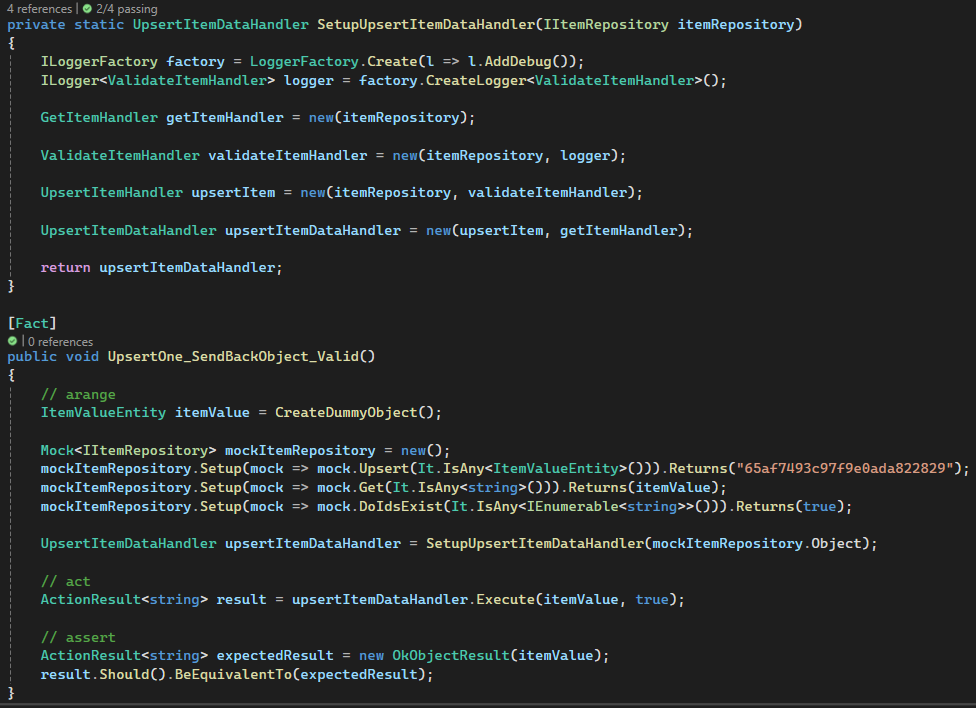
\includegraphics[scale=0.6]{IntergrationTestExample.png}
	\label{fig:IntergrationTest}
\end{graphic}

\whitespace[2]
\begin{graphic}
	\captionsetup{type=figure}
	\caption{Overzicht intergratie en unittesten}
	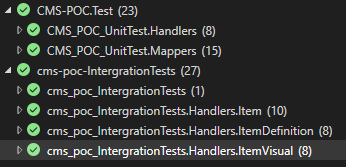
\includegraphics[scale=1]{OverzichtUnitTesten.png}
	\label{fig:OverviewUnitTests}
\end{graphic}
